\documentclass[12pt,a4paper]{article}
%\usepackage[latin1]{inputenc}
%\usepackage{achemso}
\usepackage{rsc}
\usepackage[utf8]{inputenc}
\usepackage[margin=1in]{geometry}
\usepackage{indentfirst}
\usepackage{amsmath}
%\usepackage{amsfonts}
%\usepackage{amssymb}
\usepackage{graphicx}
%\author{Ben Peyton}
\title{Notes on Richard and Herbert Many-Body Basis Set Corrections Paper\cite{Richard2013}}
\setlength{\parindent}{2em}
\begin{document}
	\maketitle
	\section{ABSTRACT}
	A method is presented of obtaining the complete basis-set (CBS) limit "based on a Boys-Bernadi-style counterpoise correction for clusters containing arbitrarily many monomer units, which is rendered computationally feasible by means of a truncated many-body expansion." cc-PVXZ basis sets are used to extrapolate to the CBS limit. A three-body expansion was shown to be within roughly 0.2 kcal/mol of traditional MP2/CBS calculations. 
	\section{BODY}
	The simplest approach for calculating the binding energy (BE) of a dimer is:
	%\begin{center}
	\begin{equation} \label{eq1}
		BE = E_{AB} - E_{A} - E_{B}
	\end{equation}
	%\end{center}
	This approach often overestimates the A-B binding energy because of the basis set superposition error (BSSE). In short, this is because the fragment $E_{AB}$ has a bigger (or more complete) basis than either monomer. If the dimer's basis functions were used for all calculations, you would arrive at the Boys-Bernadi counterpoise (CP) correction:
	\begin{equation} \label{eq2}
		BE = E_{IJK...} - \sum_{i=I,J,K...}^{N}E_{i}^{IJK...}
	\end{equation}
	where the sum is the energy of monomer i with functions on monomers I,J,K... (place ghost atoms on all monomers J$\neq$i). (Technically, the Boys-Bernardi scheme was only for dimers. This method was generalized to n-body systems by Wells \textit{et al} as the "Site-Site Function Counterpoise" or SSFC scheme\cite{Wells1983}.) In the present work this scheme is applied to a many-body expansion (MBE) to reproduce MP2/CBS limit results using a sequence of CP-corrected MP2/cc-PVXZ results. A triples correction
	\begin{equation} \label{eq3}
		\delta_{CCSD(T)} = E_{CCSD(T)} - E_{MP2}
	\end{equation}
	is also approximated with trucated MBE's.
	\newpage
	\section{MANY-BODY EXPANSION}
	The many-body expansion is used in place of each term in Eq.~\eqref{eq2} to achieve computational efficiency. The cluster energy $E_{IJK...}$ is a "traditional" MBE expression:
	\begin{equation} \label{eq4}
		E_{IJK...} = \sum_{i=1}^{N}E_{i} + \sum_{i=1}^{N}\sum_{j>i}^{N}\Delta E_{ij} + \sum_{i=1}^{N}\sum_{j>i}^{N}\sum_{k>j}^{N}\Delta E_{ijk} + ...
	\end{equation}
	\begin{subequations} 
		\begin{equation}
			\Delta E_{ij} = E_{ij} - E_{i} - E{j} \label{eq5a} \\
		\end{equation}
		\begin{equation}			
			\Delta E_{ijk} = E_{ijk} - E_{ij} - E_{ik} - E_{jk} + E_{i} + E_{j} + E_{k} \label{eq5b}
		\end{equation}
	\end{subequations}
	The monomer energies in Eq.~\eqref{eq2} contain "ghost atoms" (used to place the extra basis functions used in the counterpoise correction), and the energies associated with these ghost atoms/bodies are zero. The non-vanishing terms in the second term of Eq.~\eqref{eq2} then become
	\begin{equation}
		E_{I}^{IJ...N} = E _{I}^{I} + \Delta E_{I}^{(2)} + \Delta E_{I}^{(3)}
	\end{equation}
	$\Delta E_{I}^{(2)}$ and $\Delta E_{I}^{(3)}$ are the one- and two-body corrections to the monomer energy in the basis IJK...N from the MBE. The next two equations are given in the paper- for derivations, see \textbf{NOTES}. 
	\begin{subequations}
		\begin{equation}
			\Delta E_{I}^{(2)} = -(N-1)E_{I}^{I} + \sum_{J\neq I}^{N}E_{I}^{IJ}
		\end{equation}
		\begin{equation}
			\Delta E_{I}^{(3)} = \frac{1}{2}(N-1)(N-2)E_{I}^{I} - (N-2)\sum_{J\neq I}^{N}E_{I}^{IJ} + \sum_{J\neq I}^{N}\sum_{\substack{K>J \\ K\neq I}}^{N}E_{I}^{IJK}
		\end{equation}
	\end{subequations}
	\begin{figure}[h]
		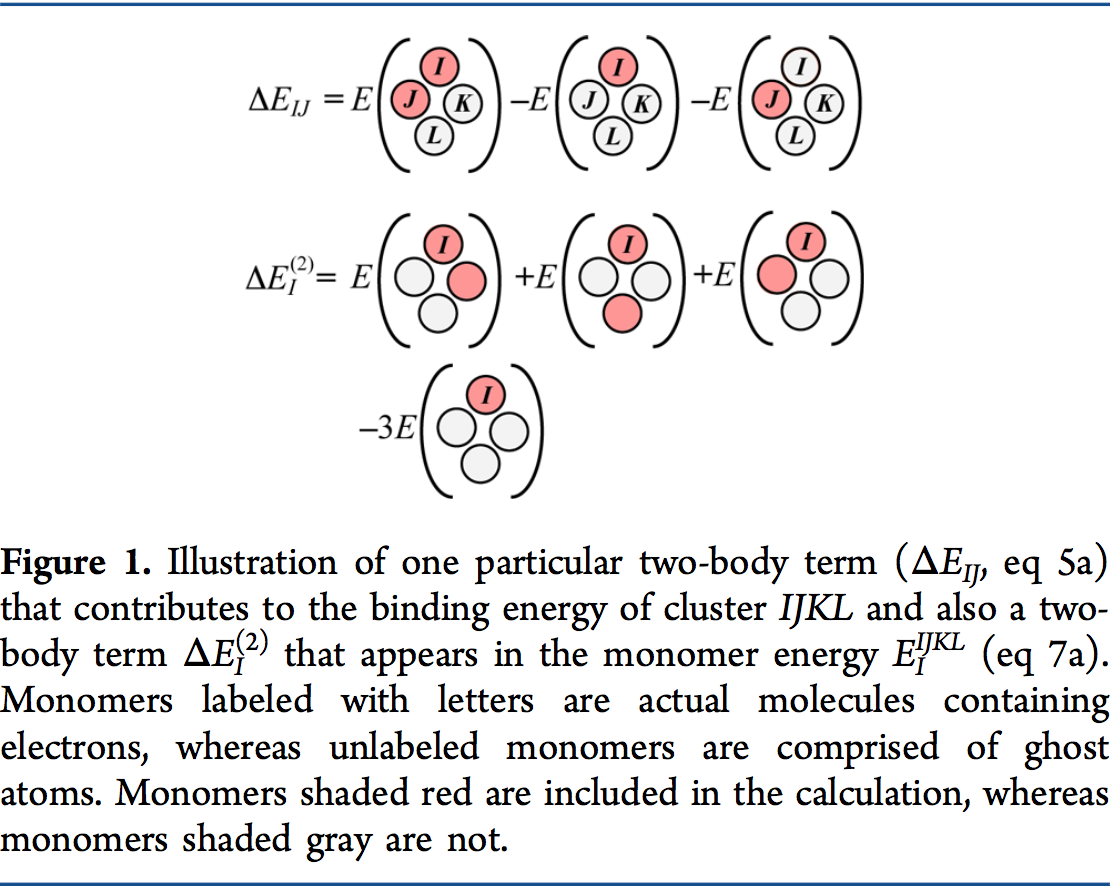
\includegraphics[scale=0.65]{Figure1.png}
		\centering
	\end{figure}
	\newpage
	\section{RESULTS}
	Using the traditional N-body expansion for the cluster energy and the CP-corrected N-body expansion for the monomer energies, the binding energy is calculated using Eq.~\eqref{eq2} truncated at "n" bodies. This is an "n-th order any-body CP correction," MBCP(n). These results are extrapolated to the CBS limit by the "traditional methods" (see the Helgaker Pink Book, 8.4.3).
	
	Extrapolating to the CBS limit should cancel out "basis set extension" error (see paper on basis set extension and Ref 8 from this paper). An alternative (but slower) CP-correction is the Valiron and Mayer function counterpoise approach (VMFC), but it grows factorially with the number of monomers. Truncated versions for two- and three-body (VMFC(2) and (VMFC(3)) were developed later.
	
	Apparently, VMFC(2) and MBPC(2) are completely equivalent (need to show this later). For n$\geq$3, MBPC(2) requires fewer calculations. Example: for n = 3, MBCP(3) requires monomer calculations in the trimer basis, while VMFC(3) requires monomer \textbf{and} dimer calculations in the trimer basis. Compared to the MBPC(2)/VMFC(2) calculations, a cluster with N = 11 monomeric units VMFC(3) requires an additional 990 calculations, while MBPC(3) requires half this number.  
	
	The two-body method MBCP(2) was not reliable, unless electrostatic embedding (EE) was used. Two systems were examined: $Gly(H_{2}O)_{10}$ and $F^{-}(H_{2}O)_{10}$. For the former, VMFC(n) and MBCP(n) were mostly comparable. MBPC(n) consistently beat out VMFC(n) results for the second more difficult system, especially with EE.
	
	EE-MBCP(3) with CBS extrapolation does an excellent job reproducing previously reported CP-MP2 CBS limit results for the "bag" isomer $(H_{2}O)_{6}$. CP-corrected and -uncorrected values are sometimes used as "error bars" for the CBS limit, but even with a quadruple basis set these "error bars" were no better than 1 kcal/mol. 
	
	A triples correction can also be employed (Eq.~\eqref{eq3}) using the many-body approximation. This was done for eight different isomers of the water hexamer $(H_{2}O)_{6}$. Using EE-MB(3) (electrostatic embedding 3-body with no counterpoise correction) with ha-TZ (aTZ without diffuse functions on H) to approximate both energies, errors of <0.01 kcal/mol were obtained relative to "true" $\delta_{CCSD}$ values (calculated for the entire hexamer, no many-body expansion) at greatly reduced cost for all eight isomers. The EE-MB(2) results were generally <0.3 kcal/mol. Using these, values can be obtained approaching the CCSD(T)-CBS limit.
\bibliographystyle{rsc}
%\bibliography{/Users/mash/Documents/Mendeley_bibtex/Many-Body.bib}
\bibliography{../Many-Body.bib}
\end{document}
